\section{Improving the Spectral Resolution of the cfCFG}
\label{sec:compensation}




%----------Characterization 1: Pileup -------------------------------
%Description of TOD contribution

\subsection{Compensating for TOD with a $4f$ pulse shaper}
%schematic of 4F pulse shaper
%good references to using an SLM to shape pulses, don't need to fully spell it out once more.

\begin{figure}
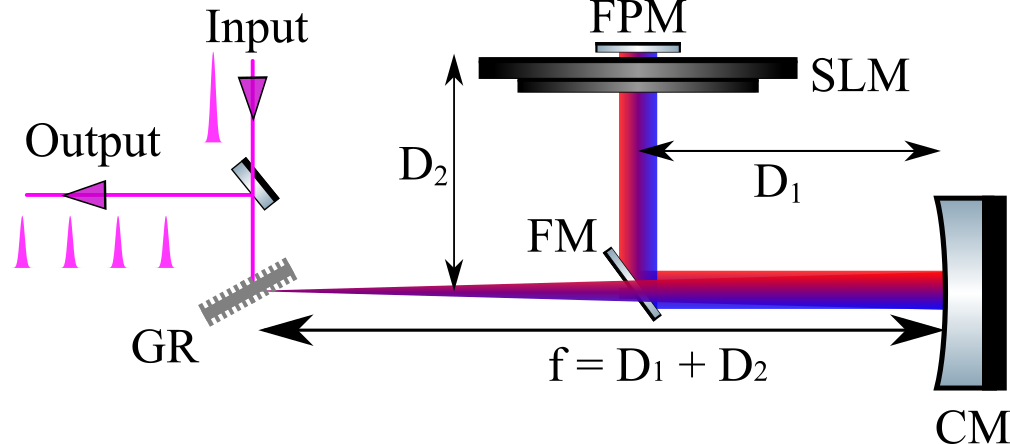
\includegraphics[width=\columnwidth]{figures/4f_folded.png}
\caption{\label{fig:4f_folded}\textcolor{red}{Will make more compact, and fix fonts. Show single chirped pulse in and out rather than the train... Should we include the Michelson afterwards? Might as well.}}
\end{figure}


%need to highlight benefits vs the method in the original spectral focusing paper, cons (energy limit from SLM)  


\subsection{Description of XCORR measurement}
%also clarify how once you've calibrated the spectrometer fit measurements this way, you can use it to directly read off the central frequency of the cfCFG and both frequency and acceleration of usCFG. 

\subsection{Demonstrating the improved resolution with Raman spectroscopy}
%mostly just need good references for how Raman works.

\begin{figure}
\includegraphics[width=\columnwidth]{figures/Raman_Setup.pdf}
\caption{\label{fig:raman_setup}\textcolor{red}{Will replace with correct font!}}
\end{figure}

%I think a single f_0 vs signal intensity scan for compensated vs uncompensated is sufficient, probably taken with oxygen at around 4x the centrifuge pulse duration? 
%Probably need 1/4 atmosphere or something to minimize collisional decoherence. 

%But the really best experiment would be showing that this makes lines resolvable with N2O, or something like that. (Since this allows for resolution greater than that of the mcpherson spectrometer!)